% This LaTeX document needs to be compiled with XeLaTeX.
\documentclass[10pt]{article}
\usepackage[utf8]{inputenc}
\usepackage{amsmath}
\usepackage{amsfonts}
\usepackage{amssymb}
\usepackage[version=4]{mhchem}
\usepackage{stmaryrd}
\usepackage{graphicx}
\usepackage[export]{adjustbox}
\graphicspath{ {./images/} }
\usepackage[fallback]{xeCJK}
\usepackage{polyglossia}
\usepackage{fontspec}

\title{第 6 章 圆锥曲线的切线 }

\author{}
\date{}


\begin{document}
\maketitle
\section*{[6.1] 过圆锥曲线上一点的切线}
\section*{(选择题)}
\begin{enumerate}
  \item 在曲线 $x y=3$ 上一点 $(1,3)$ 的切线方程式是 $\qquad$
  \item 求抛物线 $y^{2}=8 x$ 上一点 $(2,4)$ 的切线方程式
  \item 求在曲线 $x y=x+6$ 上一点 $(3,3)$ 的切线方程式。
  \item 若直线 $y=-x+c$ 切 $x y=4$, 则 $c$ 的值是 $\qquad$。
  \item 如果 $y=m x+c$ 是椭圆 $\dfrac{x^{2}}{a^{2}}+\dfrac{y^{2}}{b^{2}}=1$ 的切线, 则 $c=$ ?
  \item 求曲线 $x y=2$ 上点 $(-1,-2)$ 的切线。
  \item 求抛物线 $y^{2}=4 x+4$ 在点 $(15,8)$ 上的切线的方程式。
  \item 若 $m x+y=2$ 是抛物线 $y^{2}=6 x$ 的切线, 求此切线的斜率。
\end{enumerate}

\section*{(作答题)}
\begin{enumerate}
  \item 试证在椭圆 $\dfrac{x^{2}}{a^{2}}+\dfrac{y^{2}}{b^{2}}=1$ 上一点 $(a \cos \theta, b \sin \theta)$ 的切线与法线, 其方程式分别为
  \begin{enumerate}
    \item $\dfrac{x \cos \theta}{a}+\dfrac{y \sin \theta}{b}=1$;
    \item $\dfrac{a x}{\cos \theta}-\dfrac{b y}{\sin \theta}=a^{2}-b^{2}$.
  \end{enumerate}
  \item 试求在圆锥曲线 $x^{2}-6 x y+8 y^{2}+4 x-3 y-5=0$ 上一点 $(0,1)$ 之切线及法线方程式。
  \item 若抛物线 $y^{2}=4 x$ 在点 $P\left(t^{2}, 2 t\right)$ 的法线与抛物线交于另一点 $Q$,
 
  证明 $PQ^{2}=\dfrac{16\left(t^{2}+1\right)^{3}}{t^{4}}$ 。
  \item $y=m x+3$ 是抛物线 $y^{2}=3 x$ 的切线。在不许求 $m$ 的值的情况下, 求其切点的坐标。
  \item 证明抛物线 $y^{2}=4 x$ 上一点 $A(25,-10)$ 的法线通过 $P(21,-30)$ 。
  \item \begin{enumerate}
    \item 已知 $P(144,24)$ 及 $Q(4,4)$ 是抛物线 $y^{2}=4 x$ 上的两点。证明 $P$ 及 $Q$ 上的切线相交于抛物线 $y^{2}=8 x+4$ 上。
    \item 如果抛物线 $y^{2}=4 x$ 上另有一点 $R$ 使得弦 $PR$ 与准线平行, 求 $R$ 的坐标。
    \item 如果 $R$ 及 $Q$ 上的切线相交于另一条抛物线 $y^{2}=m-4 x$ 上, 求 $m$ 的值。
  \end{enumerate}
  \item 如果椭圆 $x^{2}+\dfrac{y^{2}}{b^{2}}=1$ 与直线 $y=x-7$ 相切, 求 $b^{2}$ 的值。
  \item 直角双曲线 $x y=c^{2}$ 上一点 $P\left(c p, \dfrac{c}{p}\right)$ 的切线交 $x$ 轴于点 $A$ 。一平行于 $y$ 轴的直线过点 $A$ 并交该直角双曲线于点 $Q$ 。另一平行于 $x$ 轴的直线过点 $P$ 并交 $y$ 轴于点 $B$ 。
  \begin{enumerate}
    \item 求点 $A$ 及点 $Q$ 的坐标;
    \item 试证 $B Q$ 为双曲线上点 $Q$ 的切线。
  \end{enumerate}
  \item 已知点 $P\left(4 p, \dfrac{4}{p}\right)$ 为直角双曲线 $x y=16$ 上的一点, 过点 $P$ 的法线分别交 $x$ 轴及 $y$轴于 $K$ 及 $L$ 两点。若 $M$ 是线段 $K L$ 的中点, 求
  \begin{enumerate}
    \item $M$ 的坐标;
    \item $M$ 的轨迹方程式。
  \end{enumerate}
  \item 求过点 $(-4,3)$ 且切抛物线 $y^{2}=4 x$ 于第一象限的切线方程。
  \item 已知抛物线 $y=x^{2}+b x+c$ 与二直线 $x+y=2$ 及 $3 x+y=4$ 相切。求
  \begin{enumerate}
    \item $b$ 及 $c$ 的值;
    \item 两个切点的坐标。
  \end{enumerate}
  \item 已知 $L_{1}$ 及 $L_{2}$ 两条直线与直线 $5 x+6 y+1=0$ 平行, 且与双曲线 $x^{2}-4 y^{2}=4$ 相切。求直线 $L_{1}$ 及 $L_{2}$ 的方程式。

  据此, 求双曲线 $x^{2}-4 y^{2}=4$ 与直线 $5 x+6 y+1=0$ 的最短距离。
  \item 直线 $y=m(x+1)$ 与抛物线 $y^{2}=4 x$ 相交于 $P\left(x_{1}, y_{1}\right)$ 及 $Q\left(x_{2}, y_{2}\right)$ 两点。
  \begin{enumerate}
    \item 以 $m$ 表示 $\left(x_{1}-x_{2}\right)^{2}$ 。
    \item 证明 $PQ^{2}=\dfrac{16\left(1+m^{2}\right)\left(1-m^{2}\right)}{m^{4}}$ 。
    \item 若 $m=\dfrac{\sqrt{2}}{2}$ 且点 $R$ 的坐标为 $(1,0)$, 利用 (b)的结果, 求 $\triangle PQR$ 的面积。
    \item 若直线 $y=m(x+1)$ 与抛物线 $y^{2}=4 x$ 相切, 求 $m$ 的值。
  \end{enumerate}
\end{enumerate}

\section*{[6.2] 已知料率的切线方程式}
\section*{(选择题)}
\begin{enumerate}
  \item 在曲线 $x y=2$ 上与直线 $y+2 x=0$ 平行的切线之方程式为 $\qquad$。
  \item 通过点 $(0,4)$ 且于第一象限切椭圆 $\dfrac{x^{2}}{4}+\dfrac{y^{2}}{9}=1$ 的切线的斜率为 $\qquad$ $\sim^{\circ}$
  \item 已知椭圆 $3 x^{2}+y^{2}=9$ 的切线的斜率是 3 , 求此切线的方程式。
  \item 求曲线 $\left\{\begin{array}{l}x=\dfrac{1}{t^{2}-1} \\ y=\dfrac{1}{\sqrt{t-1}}\end{array}, t>1\right.$, 在 $t=2$ 处的切线斜率。
  \item 求曲线 $y=\tan ^{-1} x^{2}$ 在 $x=2$ 处的切线斜率。
\end{enumerate}

\section*{(作答题)}
\begin{enumerate}
  \item 如果圆 $x^{2}+y^{2}=r^{2}$ 与椭圆 $\dfrac{x^{2}}{a^{2}}+\dfrac{y^{2}}{b^{2}}=1$ 的公切线的斜率是 $m$, 试证 $m^{2}=\dfrac{r^{2}-b^{2}}{a^{2}-r^{2}}$ 。 (3\%)由此求出圆 $x^{2}+y^{2}=25$ 与椭圆 $\dfrac{x^{2}}{16}+\dfrac{y^{2}}{169}=1$ 的公切线。
  \item 一直线通过点 $P\left(-3,-\dfrac{3}{2}\right)$, 被圆 $x^{2}+y^{2}=25$ 截得弦长为 8 单位。求此弦所在的直线的方程式。
  \item 已知 $y=4 x+c$ 与抛物线 $y^{2}=-8 x$ 相切, 求 $c$ 的值。据此, 求抛物线 $y^{2}=-8 x$ 与直线 $y=4 x-\dfrac{5}{2}$ 的最短距离。
\end{enumerate}

\section*{[6.3] 过圆锥曲线外一点的切线方程式 (选择题)}
\begin{enumerate}
  \item 从点 $(1,2)$ 到椭圆 $x^{2}+2 y^{2}=6$ 的切线是 $\qquad$。
  \item 由点 $P(-3,-8)$ 作两条切线至曲线 $y^{2}=12 x$ 。求这两条切线的斜率。
\end{enumerate}

\section*{(作答题)}
\begin{enumerate}
  \item 若直线 $y=m x+c$ 与椭圆 $\dfrac{x^{2}}{a^{2}}+\dfrac{y^{2}}{b^{2}}=1$ 相切, 试证 $c^{2}=a^{2} m^{2}+b^{2}$ 。利用以上的结果或其他方法,

(i) 求出从点 $(1,2)$ 至椭圆 $4 x^{2}+9 y^{2}=36$ 之两切线之斜率。

(ii) 若由点 $P(\alpha, \beta)$ 至椭圆 $4 x^{2}+9 y^{2}=36$ 所引之两切线互相垂直,试证 $\alpha^{2}+\beta^{2}=13$ 。
  \item 证明椭圆 $2 x^{2}+y^{2}-4 x-2 y-19=0$ 上一点 $(-2,3)$ 的切线通过点 $(1,12)$ 。并求由点 $(1,12)$ 至该椭圆的另一切线方程式。
\end{enumerate}

\section*{第7章 参数方程式}
\section*{[7.2] 参数方程和普通方程的互化}
\section*{(选择题)}
\begin{enumerate}
  \item 一曲线之参数方程式是 $x=t^{2}-2, y=t^{3}-2 t$, 求其卡氏方程式。
  \item $\left\{\begin{array}{l}x=2 \cos \theta+2 \\ y=5 \sin \theta-3\end{array}\right.$ 的正坐标方程式是
  \item 一曲线之参数方程式为 $\left\{\begin{array}{l}x=t^{2} \\ y=1-t^{4}\end{array}\right.$ 。此曲线对称于 $\qquad$。
  \item 一曲线的参数方程式是 $\left\{\begin{array}{l}x=3 \cos 2 \theta \\ y=6 \sin \theta-1\end{array}\right.$ 。这曲线的图象是 $\qquad$
  \item 参数方程 $\left\{\begin{array}{l}x=e^{t}+e^{-t} \\ y=e^{t}-e^{-t}\end{array}\right.$ 的图象是 $\qquad$。
  \item 已知参数方程式 $2 x=\sin 2 \theta, 4 y=\sin 4 \theta$, 求其卡氏方程式。
  \item 一曲线的参数方程式为 $x=\dfrac{a}{2}\left(t+\dfrac{1}{t}\right), y=\dfrac{b}{2}\left(t-\dfrac{1}{t}\right)$, 其中 $a, b$ 为常数, $t$ 为参数。试求此曲线的卡氏方程式(普通方程式)。
  \item 化参数方程式 $\left\{\begin{array}{l}x=\sin \dfrac{\alpha}{2}+\cos \dfrac{\alpha}{2} \\ y=\sin \alpha\end{array}\right.$ (式中 $\alpha$ 是参数)为卡氏方程式。
  \item 已知一曲线的参数方程式是 $x=\tan \theta, y=2 \sec \theta$ 。这曲线的图像是 $\qquad$。
  \item 参数方程式 $\left\{\begin{array}{l}x=t^{4}+t^{-4} \\ y=t^{4}-t^{-4}\end{array}\right.$ 所表示的曲线是 $\qquad$ -
\end{enumerate}

\section*{(作答题)}
\begin{enumerate}
  \item $P$ 点为 $\left(1-t^{2}, t-t^{3}\right)$, 其中 $t$ 为参数, 求 $P$ 点轨迹的卡氏方程式。
  \item 已知半圆的参数方程是 $x=\sqrt{2} \sin \theta, y^{2}=\cos 2 \theta$, 求这个半圆的半径。
  \item 求原点到曲线 $\left\{\begin{array}{l}x=-4+3 \sin \theta \\ y=3+3 \cos \theta\end{array}\right.$ ( $\theta$ 是参数) 的最短距离。
  \item 已知一曲线的参数方程式为 $\left\{\begin{array}{l}x=2+\sqrt{10} \cos \theta \\ y=1+\sqrt{10} \sin \theta\end{array}\right.$ 。此曲线与 $x$ 轴相交于 $A 、 ~B$ 两点。求

(i) 此曲线的直角坐标方程式;

(ii) 线段 $AB$ 的长。

\end{enumerate}

\section*{[7.3] 参数方程式与轨迹}
(选择题)

\begin{enumerate}
  \item $P$ 点的坐标为 $\left(3 t, t^{2}\right)$, 求 $P$ 点的轨迹方程式。
  \item 若 $P$ 为联接 $A\left(t^{2}, 0\right)$ 及 $B(0,2 t)$ 两点的直线之中点, 其中 $t$ 为参数, 则 $P$ 的轨迹为 $\qquad$。
  \item 在某变换下, $P(x, y) \rightarrow P^{\prime}(x+y, x-y)$ 。若 $P$ 点在直线 $y=2 x$ 上移动, 试求 $P^{\prime}$ 点之轨迹。
  \item 线段 $PQ$ 的长为 4 单位, 其一端点 $P$ 在 $x$ 轴上移动, 另一端点 $Q$ 在 $y$ 轴上移动。若点 $R$在 $PQ$ 上, 且 $PR: RQ=1: 3$, 试求点 $R$ 的轨迹方程式。
  \item 已知 $t$ 为任意实数, 则抛物线 $y=2 x^{2}+t x+3$ 的顶点的轨迹方程式是 $\qquad$
  \item 已知 $A(a \sec \theta, b \tan \theta)$ 是双曲线 $\dfrac{x^{2}}{a^{2}}-\dfrac{y^{2}}{b^{2}}=1$ 上的一个动点, $O$ 是原点, $P$ 是 $OA$ 的中点。求 $P$ 的轨迹方程式。
  \item 已知一动点 $P$ 到点 $(0,0)$ 的距离与其到直线 $x+y-2=0$ 的距离的比是 $1: 2$, 求 $P$ 点的轨迹方程式。
\end{enumerate}

\section*{(作答题)}
\begin{enumerate}
  \item $Q$ 为点 $(0,2), P$ 为曲线 $x=t^{2}, y=t^{3}$ 上的动点。试以 $t$ 表达 $PQ$ 中点的座标。然后求这中点的轨迹方程式。
  \item 椭圆 $x^{2}+4 y^{2}=4$ 上任一点 $T(2 \cos \theta, \sin \theta)$ 的法线与 $x$ 轴相交于 $S$, 试证 $TS$ 的中点的轨迹为 $16 x^{2}+196 y^{2}=49$ 。
  \item 若直线 $\left\{\begin{array}{l}x=1+\dfrac{1}{2} t \\ y=-3 \sqrt{3}+\dfrac{\sqrt{3}}{2} t\end{array}\right.$, 式中 $t$ 为参数, 与圆 $x^{2}+y^{2}=16$ 交于 $A$ 及 $B$ 两点, 求 $AB$中点的坐标。
  \item (a) 已知直线 $l$ 垂直于直线 $x-y+1=0$, 且与曲线 $\left\{\begin{array}{l}x=1-\dfrac{1}{1+t} \\ y=1+\dfrac{1}{t}\end{array}\right.$ ( $t$ 为参数) 只有一个交点。求直线 $l$ 的方程式。
  \item 求原点到曲线 $\left\{\begin{array}{l}x=3+2 \sin \theta \\ y=-4+2 \cos \theta\end{array}\right.$ ( $\theta$ 为参数) 上的最短距离。
  \item 右如图所示, $P(a \sec \theta, b \tan \theta)$ 为双曲线 $\dfrac{x^{2}}{a^{2}}-\dfrac{y^{2}}{b^{2}}=1$ 上的一点; $PN$ 为过点 $P$ 的法线, $PN$ 与 $x$ 轴相交于点 $N, M$ 为 $PN$ 的中点。

\begin{enumerate}
  \item 证明 PN 的方程式为

  $$
  y=-\dfrac{a \sin \theta}{b} x+\dfrac{a^{2}+b^{2}}{b} \tan \theta
  $$
  
  \item 求点 $M$ 的轨迹的直角坐标方程式,并说明它是哪一类的圆锥曲线。
\end{enumerate}

\begin{center}
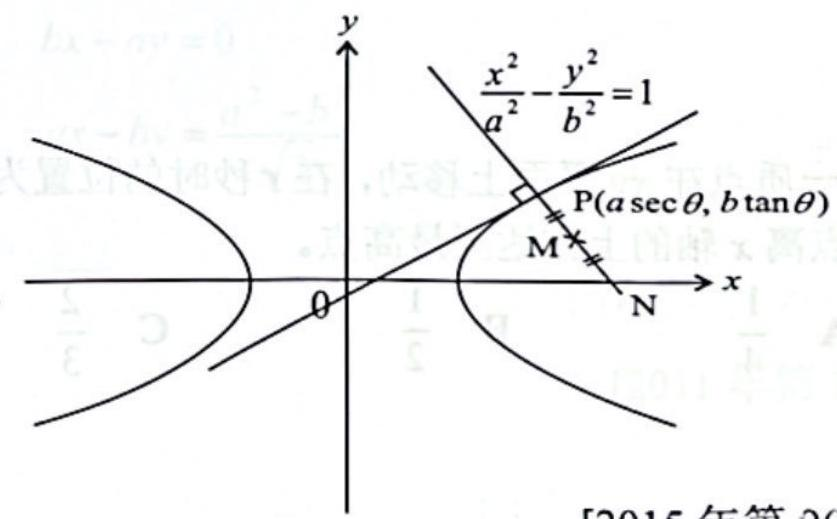
\includegraphics[max width=\textwidth]{2024_06_05_971e6815482d5ecd2718g-10}
\end{center}

\end{enumerate}


\section*{[7.4] 参数函数的微分法}
(选择题)

\begin{enumerate}
  \item $PQ$ 是抛物线 $y^{2}=4 a x$ 的一焦弦, 则在 $P$ 和 $Q$ 的切线交于直线
  \item 已知 $y=4-3 t^{2}$ 及 $x=t^{2}-t+1$, 求 $\dfrac{d y}{d x}$ 当 $t=-1$ 。
  \item 若 $\left\{\begin{array}{l}x=t+\sin t \\ y=\cos t\end{array}\right.$, 求 $\dfrac{d y}{d x}$ 。
  \item 求函数 $\left\{\begin{array}{l}y=\ln t \\ x=1+t^{2}\end{array}\right.$ 之 $\dfrac{d y}{d x}$ 。
  \item 一曲线之参数方程式为 $\left\{\begin{array}{l}x=2 \cos ^{3} t \\ y=\sin ^{3} t\end{array}\right.$ 。求 $\dfrac{d y}{d x}$, 以 $t$ 表示之。
  \item 一质点在 $x y$ 平面上移动, 在 $t$ 秒时的位置为 $x=t+t^{2}, y=t-t^{2}$ 。当 $x=$ $\qquad$时, 质点离 $x$ 轴的上方达至最高点。
  \item 若 $y=\cos 2 t$ 及 $x=\sin t$, 求此曲线在点 $t=\dfrac{\pi}{6}$ 的法线方程式。
  \item 一曲线的参数方程式为 $\left\{\begin{array}{l}x=\sin \theta \\ y=2 \cos \theta\end{array}\right.$ 。当 $\theta=\dfrac{3}{4} \pi$, 求 $\dfrac{d y}{d x}$ 的值。
  \item 一质点在 $x y$ 平面上移动。在 $t$ 秒时它的位置是 $x=\left(t^{2}+1\right) m, y=(t-1) m$ 。试求它在 $t=10$ 秒时的速率。
  \item 一曲线的参数方程式是 $\left\{\begin{array}{l}x=a t^{2} \\ y=2 a t\end{array}\right.$ 。求曲线在 $t=2$ 时的点的法线方程式。
  \item 求在曲线 $\left\{\begin{array}{l}x=\dfrac{2 t}{1+t^{2}} \\ y=\dfrac{1-t^{2}}{1+t^{2}}\end{array}\right.$ 上 $t=2$ 处的切线方程式。
  \item 一曲线的参数方程式为 $x=a \cos \theta, y=b \sin \theta$ 。求在点 $\theta=\dfrac{\pi}{4}$ 的法线方程式。
  \item 已知 $\left\{\begin{array}{l}x=t^{2}+t \\ y=t^{3}\end{array}\right.$, 求 $\dfrac{d^{2} y}{d x^{2}}$ 。
  \item 已知 $\left\{\begin{array}{l}x=\cos t+t \sin t \\ y=\sin t-t \cos t\end{array}\right.$, 求 $\dfrac{d^{2} y}{d x^{2}}$ 。
\end{enumerate}

\section*{(作答题)}
\begin{enumerate}
  \item 已知一参数方程式 $\left\{\begin{array}{l}x=2 t^{2}-t \\ y=t^{2}+1\end{array}\right.$, 求当 $x=1, y=2$ 时 $\dfrac{d y}{d x}$ 之值。
  \item 一曲线的参数方程式为 $\left\{\begin{array}{l}x=2 \cos 2 \theta+1 \\ y=\sin \theta+2\end{array}\right.$ 。求
  \begin{enumerate}
    \item 此曲线的直角坐标方程式;
    \item 此曲线在点 $\theta=\dfrac{\pi}{6}$ 上的法线方程式。
  \end{enumerate}
  \item 一曲线的参数方程式为 $\left\{\begin{array}{l}x=t^{2} \\ y=t^{3}\end{array}\right.$ 。试描绘此曲线的图象。
  \begin{enumerate}
    \item 求此曲线的直角坐标方程式。
    \item 求曲线上 $A(4,8)$ 点的法线方程式。
    \item 已知 $O$ 为原点, $N$ 为法线 $AN$ 与 $x$ 轴的交点, 求由曲线 $OA$, 法线 $AN$ 及 $x$ 轴所围成的区域的面积。
    \item 求此面积绕 $x$ 轴旋转一周所形成的体积。
  \end{enumerate}
  \item 已知一曲线的参数是 $x=a t^{3}, y=b t^{2}$ 式中 $a, b$ 为正的常数。过点 $T\left(a t^{3}, b t^{2}\right)$ 的切线交 $y$轴于 $Y, M$ 是从点 $T$ 到 $y$ 轴的垂足。证明 $OM=3 OY, O$ 为原点。
  \item 已知 $x=\theta-\sin \theta, y=1-\cos \theta$, 求 $\dfrac{d^{2} y}{d x^{2}}$ 。
  \item 若一曲线的参数方程式为 $\left\{\begin{array}{l}x=3 \cos \theta-2 \cos ^{3} \theta \\ y=2 \sin ^{3} \theta\end{array}\right.$, 试证曲线过一参数为 $\theta$ 的点的法线方程式为 $x \cos 2 \theta+y \sin 2 \theta=\cos \theta$ 。
  \item 已知参数方程式 $\left\{\begin{array}{l}x=\theta-\cos \theta \\ y=1+\sin \theta\end{array}\right.$, 其中 $0<\theta<2 \pi$, 试证 $\dfrac{d^{2} y}{d x^{2}}=-\dfrac{1}{y^{2}}$ 。
  \item 抛物线 $y^{2}=4 a x$ 上一点 $P\left(a t^{2}, 2 a t\right)$ 的切线与 $x$ 轴相交于点 $A$, 过点 $P$ 的法线则与 $x$ 轴相交于点 $B$ 。过点 $P$ 的切线与直线 $OP$ 的夹角是 $\theta$, 其中 $O$ 为原点, $\theta$ 为锐角。
  \begin{enumerate}
    \item 求点 $A$ 及点 $B$ 的坐标;
    \item 证明三角形 $ABP$ 的面积为 $\left|2 a^{2} t\left(1+t^{2}\right)\right|$;
    \item 证明 $\tan \theta=\dfrac{t}{t^{2}+2}$ 。
  \end{enumerate}
  \item 已知参数方程式 $\left\{\begin{array}{l}x=a(\theta-\sin \theta) \\ y=a(1-\cos \theta)\end{array}\right.$, 求当 $\theta=\dfrac{\pi}{3}$ 时 $\dfrac{d^{2} y}{d x^{2}}$ 的值。
\end{enumerate}

\section*{[7.5] 圆锥曲线的参数方程式}
\section*{(选择题)}
\begin{enumerate}
  \item 假设 $Q$ 是圆 $x^{2}+y^{2}=4$ 上的动点, 点 $R$ 的坐标是 $(4,0)$, 则 $RQ$ 的中点的轨迹方程式是 $\qquad$。
  \item 求抛物线 $x^{2}=\dfrac{1}{4} y$ 上一点的坐标, 此点到直线 $y=4 x-5$ 的距离最短。
  \item 如右图所示, 一焦点为 $F_{1}$ 及 $F_{2}$ 的椭圆经过 $A, B, C, D$ 四点。若 $A B F_{1} C D F F_{2}$ 为一正六边形, 求此椭圆的离心率。
  \begin{center}
    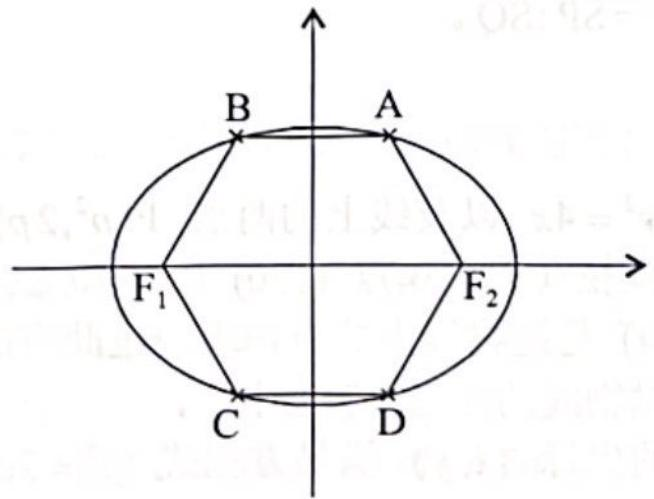
\includegraphics[max width=\textwidth]{2024_06_05_971e6815482d5ecd2718g-14}
  \end{center}
\end{enumerate}

\section*{(作答题)}
\section*{抛物线}
\begin{enumerate}
  \item \begin{enumerate}
    \item 抛物线 $x=a t^{2}, y=2 a t$ 上的两点的参数为 $t=t_{1}$ 及 $t=t_{2}$ 。试证明通过这两点的弦的方程式是 $y=\dfrac{2}{t_{1}+t_{2}} x+\dfrac{2 a t_{1} t_{2}}{t_{1}+t_{2}}$ 。由此, 或用其他方法, 求这拔物线在点的参数为 $t$ 的切线及法线方程式。

    \item 抛物线 $x=a t^{2}, y=2 a t$ 在点的参数为 $t=t_{0}$ 的法线交这抛物线于另一点 $P$, 试证 $P$ 点的参数是 $-\dfrac{2}{t_{0}}-t_{0}$ 。
  \end{enumerate}

  \item 抛物线 $y^{2}=4 a x$ 在点 $P\left(a p^{2}, 2 a p\right)$ 及点 $Q\left(a q^{2}, 2 a q\right)$ 之切线相交于 $R$, 试求 $R$ 之坐标, 并证 $\triangle PQR$ 之面积为 $\left|\dfrac{1}{2} a^{2}(p-q)^{3}\right|$ 。
  \item 求抛物线 $y^{2}=4 a x$ 在点 $P\left(a t^{2}, 2 a t\right)$ 的切线方程式. 已知过原点 $O$ 而平行于此切线之直线交此抛物线于 $Q$ 。试证过 $P$ 点而平行于抛物线轴之直线通过 $O Q$ 之中点。
  \item 过抛物线 $y^{2}=4 a x$ 上一点 $P\left(a p^{2}, 2 a p\right)$ 所作的法线与抛物线重交于 $Q\left(a q^{2}, 2 a q\right)$ 点, 求 $p$ 与 $q$ 之间的代数关系式, 并证明 $q^{2} \geq 8$ 。证明弦 $PQ$ 之长度为 $\dfrac{4 a\left(1+p^{2}\right)^{\dfrac{3}{2}}}{p^{2}}$ 。
  \item $P\left(a p^{2}, 2 a p\right)$ 为抛物线 $y^{2}=4 a x$ 上一点, 且 $S(a, 0)$ 为抛物线的焦点。求 $\triangle PSQ$ 的最大值, 其中 $Q$ 点为直线 $y=-2 a t$ 和抛物线的交点。

  试证 $SP=a\left(p^{2}+1\right)$ 。

  若此抛物线上的两点 $P$ 与 $Q$ 其切线相交于 $T$ 。试证:
        \begin{enumerate}
            \item $ST^{2}=SP \cdot SQ$ 。
            \item $TP^{2}: TQ^{2}=SP: SQ$ 。
        \end{enumerate}
    
    \item 给出抛物线 $y^{2}=4 x$ 以及线上的两点 $P\left(p^{2}, 2 p\right)$ 与 $Q\left(q^{2}, 2 q\right)$ 。
        \begin{enumerate}
            \item 若 $PQ$ 为焦弦 (通过焦点 $(1,0)$ 的弦), 试证 $p q=-1$ 。
            \item 已知 $(4,4)$ 是抛物线上的点, 求通过此点的焦弦之长度。
            \item 若 $M$ 是抛物线的焦弦 $PQ$ 之中点,试证 $M$ 的坐标 $(x, y)$ 满足方程式 $y^{2}=2(x-1)$ 。
        \end{enumerate}

    \item 试证明过抛物线 $y^{2}=4 a x$ 上一点 $P\left(a t^{2}, 2 a t\right)$ 所作切线其方程式为 $t y-x-a t^{2}=0$ 。

    若过 $P$ 点的切线及法线分别交 $x$ 轴于 $T$ 点及 $N$ 点, 试证明:
        \begin{enumerate}
            \item $\dfrac{PT}{PN}=|t|$,
            \item $PT \cdot PN=\left|4 a^{2} t\left(1+t^{2}\right)\right|$ 。
        \end{enumerate}

    \item $P\left(a p^{2}, 2 a p\right), Q\left(a q^{2}, 2 a q\right)$ 及 $R\left(a r^{2}, 2 a r\right)$ 是抛物线 $y^{2}=4 a x$ 上之三个不同点。试证:
        \begin{enumerate}
            \item 在 $P$ 点上抛物线之法线其方程式为 $y=-p x+2 a p+a p^{3}$;
            \item 在 $P$ 及 $Q$ 两点上抛物线之法线其交点为 $\left(2 a+a p^{2}+a q^{2}+a p q,-a p q(p+q)\right)$;
            \item 若在 $P, Q$ 及 $R$ 三点上抛物线之法线共点, 则 $p+q+r=0$ 。
        \end{enumerate}

  \item $P\left(a p^{2}, 2 a p\right)$ 及 $Q\left(a q^{2}, 2 a q\right)$ 是抛物线 $y^{2}=4 a x$ 上相异的两点。若直线 $PQ$ 通过点 $(2 a, 0)$,

  试证 \begin{enumerate}
    \item $p q=-2$;

    \item 抛物线在 $P$ 及 $Q$ 两点上的切线相交于直线 $x=-2 a$ 上。
  \end{enumerate}

  \item 一曲线的参数方程式为 $\left\{\begin{array}{l}x=t^{2}-1 \\ y=4 t\end{array}\right.$ 。试求
  \begin{enumerate}
    \item 曲线在 $x=0$ 的点上两切线之方程式及其交点的坐标;
    \item 此曲线的直角坐标方程式;
    \item 其焦点的坐标。
  \end{enumerate}

  \item \begin{enumerate}
  \item 试证自点 $(42,-60)$ 可引三条不同的法线至抛物线 $y^{2}=8 x$ 。求此三条法线之方程式。

  \item 自点 $\left(x_{0}, y_{0}\right)$ 引法线至抛物线 $y^{2}=4 a x$, 交抛物线于点 $\left(x_{1}, y_{1}\right),\left(x_{2}, y_{2}\right)$ 及 $\left(x_{3}, y_{3}\right)$, 试证
  \begin{enumerate}
    \item $y_{1}+y_{2}+y_{3}=0$;
    \item $x_{1}+x_{2}+x_{3}=2\left(x_{0}-2 a\right)$ 。
  \end{enumerate}
 \end{enumerate}

  \item \begin{enumerate}
    \item $P\left(a t^{2}, 2 a t\right)$ 是抛物线 $y^{2}=4 a x$ 上的一点。试证在 $P$ 点的切线的方程式是 $t y=x+a t^{2}$ 。

    \item $A\left(a t_{1}^{2}, 2 a t_{1}\right)$ 及 $B\left(a t_{2}^{2}, 2 a t_{2}\right)$ 是抛物线 $y^{2}=4 a x$ 上两点。 $O$ 是原点, 且 $\angle AOB=90^{\circ}$ 。
    \begin{enumerate}
      \item 试证在 $A$ 及 $B$ 上的切线相交于 $T\left(a t_{1} t_{2}, a\left(t_{1}+t_{2}\right)\right)$ 点, 此点落在直线 $x+4 a=0$ 上。
      \item 如果 $M$ 是 $AB$ 的中点, 试证 $M$ 落在曲线 $y^{2}=2 a(x-4 a)$ 上。
    \end{enumerate}
  \end{enumerate}

  \item $P\left(a p^{2}, 2 a p\right)$ 是抛物线 $y^{2}=4 a x$ 上的一点。证过 $P$ 点的法线其方程式为 $y+p x=2 a p+a p^{3}$ 。如果这条法线再交抛物线于点 $Q\left(a q^{2}, 2 a p\right)$, 证 $q=-p-\dfrac{2}{p}$ 。

  如果 $Q$ 点的法线又交抛物线于点 $R\left(a r^{2}, 2 a r\right)$, 证 $r=p+\dfrac{2}{p}+\dfrac{2 p}{p^{2}+2}$ 。

  \item 试证在抛物线 $y^{2}=4 a x$ 上一点 $P\left(a t^{2}, 2 a t\right)$ 的法线方程式为 $y+t x=2 a t+a t^{3}$ 。此法线交 $x$轴于 $G$ 且 $P G$ 的中点为 $M$ 。
  \begin{enumerate}
    \item 若 $P$ 点沿抛物线移动, 求 $M$ 点的轨迹方程式。
    \item 若此抛物线的焦点为 $S$, 试证 $\angle PMS=90^{\circ}$ 。
    \item 若 SPG 为一等边三角形, 求 $P$ 点的坐标。
  \end{enumerate}

  \item 试证在抛物线 $y^{2}=4 a x$ 上两点 $P\left(a p^{2}, 2 a p\right)$ 及 $Q\left(a q^{2}, 2 a q\right)$ 的切线的交点为 $T(a p q, a(p+q))$ 。

  设在 $P$ 与 $Q$ 两点上的切线分别与 $y$ 轴相交于 $R$ 与 $S$ 。
  \begin{enumerate}
    \item 试求 $R$ 及 $S$ 的坐标。
    \item 试证 $\Delta RST$ 的面积为 $\dfrac{1}{2} a^{2}|p q(q-p)|$ 。
    \item 若线段 RS 之长为 $k$, 试证 $T(a p q, a(p+q))$ 落在曲线 $y^{2}-4 a x=k^{2}$ 上。
  \end{enumerate}

  \item 证明抛物线 $y^{2}=4 a x$ 在点 $P\left(a p^{2}, 2 a p\right)$ 的法线方程式为 $y+p x=2 a p+a p^{3}$ 。
  \begin{enumerate}
    \item 若此法线再交抛物线于点 $Q\left(a q^{2}, 2 a q\right)$, 证明 $p^{2}+p q+2=0$, 并推断 $q^{2}$ 不能少于 8 。
    \item 若 $\angle POQ=90^{\circ}, O$ 为原点, 求点 $P$ 与 $Q$ 的坐标。
  \end{enumerate}

  \item 若抛物线 $y^{2}=4 x$ 在点 $P\left(t^{2}, 2 t\right)$ 的法线与抛物线交于另一点 $Q$,证明 $P Q^{2}=\dfrac{16\left(t^{2}+1\right)^{3}}{t^{4}}$ 。

  \item \begin{enumerate}
    \item 已知 $P\left(p^{2}, 2 p\right)$ 及 $Q\left(q^{2}, 2 q\right)$ 是抛物线 $y^{2}=4 x$ 上两点, 证明
    \begin{enumerate}
      \item $P$ 及 $Q$ 的切线交于 $R(p q, p+q)$;
      \item 直线 $PQ$ 的方程式是 $(p+q) y=2 x+2 p q$ 。
    \end{enumerate}
  
    \item 过 $R$ 点及原点 $O$ 的直线 $RO$ 交 $PQ$ 于 $N$ 。
    \begin{enumerate}
      \item 若 $P$ 点及 $Q$ 点沿着抛物线移动且 $p q$ 的值恒是 -2 时, 证明 $N$ 为
      $$
      \left(\dfrac{8}{4+(p+q)^{2}}, \dfrac{-4(p+q)}{4+(p+q)^{2}}\right)
      $$
      \item 由此, 证明 $N$ 的轨迹是一个圆。
    \end{enumerate}
  \end{enumerate}

  \item $P\left(a p^{2}, 2 a p\right)$ 及 $Q\left(a q^{2}, 2 a q\right)$ 在抛物线 $y^{2}=4 a x$ 上, $M$ 是 $PQ$ 的中点。

  \begin{enumerate}
    \item 试证在抛物线上 $P$ 及 $Q$ 的切线的交点是 $T(a p q, a(p+q))$;

    \item 若弦 $PQ$ 对顶点的张角为一直角, 证明 $p q=-4$;
    
    \item 据此, 或用其他方法, 证明 $M$ 的轨迹方程式是 $y^{2}=2 a(x-4 a)$ 。
  \end{enumerate}

  \item 求通过点 $(15,-3)$ 至抛物线 $y^{2}=16 x$ 的法线。

  \item 抛物线 $y=x^{2}$ 与圆相切于点 $P\left(t, t^{2}\right)$, 且圆的半径是 $\sqrt{1+4 t^{2}}$ 。求抛物线上过点 $P$ 的法线方程式。

据此, 或用其他方法, 证明圆心的轨迹方程式是 $y=x^{2}+1$ 或 $y=\dfrac{x^{2}}{9}-1$ 。

  \item 如右图所示, $P$ 是抛物线 $y=x^{2}$ 上的动点。若以 $O P$ 为一边, 作正方形 $O P Q R$,且 $R$ 亦是此抛物线上的动点, 求 $Q$ 点的轨迹。

\begin{center}
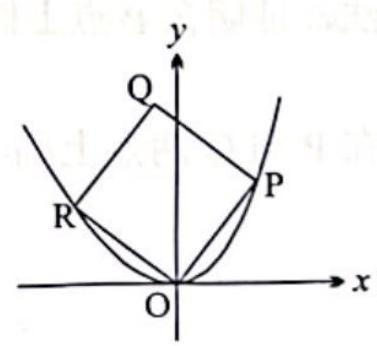
\includegraphics[max width=\textwidth]{2024_06_05_971e6815482d5ecd2718g-18}
\end{center}

\end{enumerate}

椭圆

\begin{enumerate}
  \item $P$ 与 $Q$ 为椭圆 $\dfrac{x^{2}}{a^{2}}+\dfrac{y^{2}}{b^{2}}=1$ 上的二点, 其坐标分别为 $(a \cos \theta, b \sin \theta)$ 及 $(-a \sin \theta, b \cos \theta)$ 。 $O$ 为原点, 试证

  \begin{enumerate}
    \item $OP^{2}+OQ^{2}=a^{2}+b^{2}$;
    \item 三角形 $OPQ$ 之面积为 $\dfrac{1}{2} a b$;
    \item $PQ$ 之中点落于椭圆 $\dfrac{2 x^{2}}{a^{2}}+\dfrac{2 y^{2}}{b^{2}}=1$ 上。
  \end{enumerate}

  \item 已知椭圆 $\dfrac{x^{2}}{a^{2}}+\dfrac{y^{2}}{b^{2}}=1(a>b)$ 及其上两点 $P$ 与 $Q$,

  \begin{enumerate}
    \item 试证 $\triangle OPQ$ 之面积 $\leq \dfrac{1}{2} a b$, 其中 $O$ 为原点;
    \item 若 $P$ 点上之法线交长轴于 $G$, 试证 $PG$ 平分 $\angle SPS^{\prime}$, 其中 $S, S^{\prime}$ 为椭圆之两焦点。
  \end{enumerate}

  \item \begin{enumerate}
    \item 若直线 $y=m x+c$ 与椭圆 $\dfrac{x^{2}}{9}+\dfrac{y^{2}}{4}=1$ 相切, 试求 $c$ 与 $m$ 之关系式。
    \item 若由 $P$ 点至椭圆 $\dfrac{x^{2}}{9}+\dfrac{y^{2}}{4}=1$ 所引两切线互相垂直, 应用(a), 试写出此二切线以 $m$ 表示之方程式, $m$ 为其中一切线之斜率。
  
    然后, 或用其他方法, 证明当 $m$ 变化时, $P$ 点之轨迹为一半径为 $\sqrt{13}$ 之圆。
  \end{enumerate}

  \item $P(3 \cos \theta, 2 \sin \theta)$ 及 $Q(3 \cos \phi, 2 \sin \phi)$ 为椭圆 $\dfrac{x^{2}}{9}+\dfrac{y^{2}}{4}=1$ 上之两点。

  试证 $PQ$ 之斜率为 $-\dfrac{2}{3} \cot \dfrac{\theta+\phi}{2}$ 。

  以此或其他方法, 证明在 $P$ 点上椭圆之切线其方程式为 $3 y \sin \theta+2 x \cos \theta=6$ 。

  此外, 再证明在 $P$ 与 $Q$ 两点上椭圆的切线之交点为 $\left(\dfrac{3 \cos \dfrac{1}{2}(\phi+\theta)}{\cos \dfrac{1}{2}(\phi-\theta)}, \dfrac{2 \sin \dfrac{1}{2}(\theta+\phi)}{\cos \dfrac{1}{2}(\theta-\phi)}\right)$ 。

  \item $P(2 \cos t, \sin t)$ 是椭圆 $\dfrac{x^{2}}{4}+y^{2}=1$ 上的一点。求过 $P$ 点的法线之方程式。这条法线交 $y$轴于点 G。M 是 $P G$ 的中点。当 $t$ 变化时, 求 $M$ 的轨迹。

  \item 试证椭圆 $\dfrac{x^{2}}{a^{2}}+\dfrac{y^{2}}{b^{2}}=1$ 上一点 $P(a \cos \theta, b \sin \theta)$ 的法线方程式为 $\dfrac{a x}{\cos \theta}-\dfrac{b y}{\sin \theta}=a^{2}-b^{2}$ 。

  若过点 $P$ 的法线交 $x$ 轴於 $G$, 证明 $OG=e^{2} ON$, 式中 $O$ 为原点, $e$ 为椭圆离心率, $N$ 为在 $x$ 轴上的 $P$ 的垂足。

  \item \begin{enumerate}
    \item 已知点 $P(2,2)$ 是椭圆 $x^{2}+4 y^{2}-2 x-12 y+6=0$ 的一条弦的中点。求这条弦的方程式。

    \item 试证在椭圆 $\dfrac{x^{2}}{a^{2}}+\dfrac{y^{2}}{b^{2}}=1$ 上一点 $P(a \cos \theta, b \sin \theta)$ 的法线方程式为 $a x \sin \theta-b y \cos \theta=\left(a^{2}-b^{2}\right) \sin \theta \cos \theta$ 。
  
    若此法线交 $x$ 轴于 $A$, 交 $y$ 轴于 $B$, 试证三角形 $OAB$ 的面积不能大过 $\dfrac{\left(a^{2}-b^{2}\right)^{2}}{4 a b}$, $O$ 为原点。
  \end{enumerate}

  \item \begin{enumerate}
    \item 在椭圆 $\dfrac{x^{2}}{a^{2}}+\dfrac{y^{2}}{b^{2}}=1$ 上的两点 $P$ 及 $Q$ 的坐标分别是 $(a \cos \theta, b \sin \theta)$ 及 $(-a \sin \theta, b \cos \theta)$ 。
    
    \begin{enumerate}
      \item 若$O$是原点,试证明
      \begin{enumerate}
        \item $OP^{2}+OQ^{2}=a^{2}+b^{2}$;
        \item 三角形 $OPQ$ 的面积是 $\dfrac{1}{2} a b$ 。
      \end{enumerate}
    
    \item 当 $P$ 及 $Q$ 变动时, 求 $PQ$ 中点的轨迹方程式。
    \end{enumerate}
  
  \item 点 $S$ 及 $T$ 的坐标分别是 $(0, \beta)$ 及 $(\alpha, 0)$ 。 $ST$ 的长度是 $9 ~m$ 。点 $R(x, y)$ 将 $ST$ 内分成 $1: 2$ 。当 $S$ 及 $T$ 分别在两坐标轴上移动, 求 $R$ 点的轨迹方程式。
  \end{enumerate}

\item \begin{enumerate}
  \item 试证连接椭圆 $\dfrac{x^{2}}{a^{2}}+\dfrac{y^{2}}{b^{2}}=1$ 上的两点 $P(a \cos \theta, b \sin \theta)$ 和 $Q(a \cos \phi, b \sin \phi)$ 的弦的方程式是 $\dfrac{x}{a} \cos \dfrac{\theta+\phi}{2}+\dfrac{y}{b} \sin \dfrac{\theta+\phi}{2}=\cos \dfrac{\theta-\phi}{2}$ 。

  \item 若弦 PQ 与圆 $x^{2}+y^{2}=b^{2}$ 相切, 试证 $a^{2} \cos ^{2} \dfrac{\theta-\phi}{2}=b^{2} \cos ^{2} \dfrac{\theta+\phi}{2}+a^{2} \sin ^{2} \dfrac{\theta+\phi}{2}$ 。
  
  \item 据此,或其他方法,若 $\sin(\theta-\phi) \geq 0$,证明 $PQ = a \sin(\theta-\phi)$ 。
\end{enumerate}

\item 已知点 $A(1,3)$ 在椭圆 $\dfrac{x^{2}}{4}+\dfrac{y^{2}}{12}=1$ 上, 过 $A$ 点, 作两条直线与椭圆相交于 $B, C$ 两点。若直线 $AB, AC$ 与 $x$ 轴所围成的三角形为等腰三角形, 其中 $\angle BAC$ 为顶角。求
  \begin{enumerate}
    \item 直线 $BC$ 的斜率;
    \item $\triangle ABC$ 的面积, 若 $B$ 点落在正 $x$ 轴上。
  \end{enumerate}

\item 试证椭圆 $\dfrac{x^{2}}{a^{2}}+\dfrac{y^{2}}{b^{2}}=1$ 上一点 $(a \cos \theta, b \sin \theta)$ 的切线方程式为 $\dfrac{x \cos \theta}{a}+\dfrac{y \sin \theta}{b}=1$ 。据此, 或用其他方法, 若 $P(x, y)$ 为椭圆 $4 x^{2}+9 y^{2}-36=0$ 上的一点, 求 $2 x+3 y$ 的最大值与最小值。

\item 已知一椭圆的方程式为 $x^{2}+4 y^{2}-6 x-16 y+21=0$ 。
  \begin{enumerate}
    \item 求椭圆的中心 $O^{\prime}$ 的坐标及椭圆的参数方程式。
    \item 若 $A, B$ 为椭圆上的点且线段 $AB$ 平行于 $y$ 轴, 证明 $\Delta O^{\prime} AB$ 的最大可能面积为 1 。
  \end{enumerate}

\item 求椭圆 $9 x^{2}+4 y^{2}-36 x+8 y+4=0$ 的参数方程式。据此, 或用其他方法, 若 $(\alpha, \beta)$ 为椭圆 $9 x^{2}+4 y^{2}-36 x+8 y+4=0$ 上的点, 求 $\alpha+3 \beta$ 的最大值。

\item 如右图所示, $P(a \cos \theta, b \sin \theta)$ 是椭圆 $\dfrac{x^{2}}{a^{2}}+\dfrac{y^{2}}{b^{2}}=1$ 上的一点, $O$ 及 $F$ 分别是椭圆的中心及焦点。直线 $l_{1}$ 切椭圆于点 $P$, 直线 $l_{2}$经过焦点且与 $l_{1}$ 互相垂直。点 $T$ 是 $OP$ 与 $l_{2}$的交点。设 $e$ 为椭圆的离心率。
\begin{center}
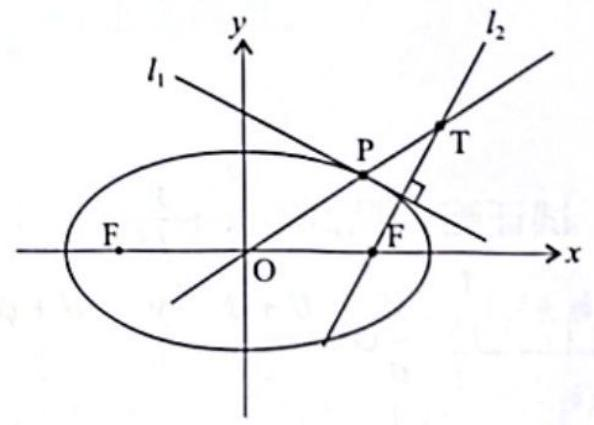
\includegraphics[max width=\textwidth]{2024_06_05_971e6815482d5ecd2718g-21}
\end{center}
  \begin{enumerate}
    \item 用微分法证明切线 $l_{1}$ 的方程式是 $\dfrac{x \cos \theta}{a}+\dfrac{y \sin \theta}{b}=1$ 。
    \item 求直线 $l_{2}$ 与直线 OP 的方程式;
    \item 证明点 $T$ 的轨迹方程式是 $x=\dfrac{a}{e}$ 。
  \end{enumerate}

\end{enumerate}

\section*{双曲线和直角双曲线}
\begin{enumerate}
  \item $P$ 和 $Q$ 为双曲线 $x y=c^{2}$ 上任意两点。 $PQ$ 之中点为 $M$ 。在点 $P$ 及点 $Q$ 上之两切线相交于 $T$ 。试证
  \begin{enumerate}
    \item 直线 MT 经过原点;
    \item 直线 $M T$ 和 $P Q$ 与 $x$ 轴之交角相等;
    \item 若 $P$ 与 $Q$ 的位置变动时, $T$ 皆落于一固定直线 $y=k(k \neq 0)$ 上, 则 $M$ 必在另一个固定直线 $x=\dfrac{c^{2}}{k}$ 上。
  \end{enumerate}
  
  \item \begin{enumerate}
    \item 直线 $y=2 x+3$ 交双曲线 $x y=c^{2}$ 于 $P$ 及 $Q$ 两点。试求 $PQ$ 中点的坐标。

    \item 试求双曲线 $x y=16$ 的一切线, 它通过点 $(0,4)$, 并求其切点的坐标。
  \end{enumerate}

  \item 试证过双曲线 $x y=c^{2}$ 上一点 $\left(x_{1}, y_{1}\right)$ 之切线的方程式可写成 $\dfrac{x}{2 x_{1}}+\dfrac{y}{2 y_{1}}=1$ 。如果此切线交坐标轴于 $A$ 及 $B$ 两点, 且 $O$ 为原点, 试证 $\triangle O A B$ 的面积是一个常数。
  
  \item 若点 $M(x, y)$ 是正双曲线 $x y=a^{2}$ 上 $PQ$ 弦的中点, 且 $P, Q$ 两点分别为 $\left(a p, \dfrac{a}{p}\right)$ 及 $\left(a q, \dfrac{a}{q}\right)$,证 $p+q=\dfrac{2 x}{a}$ 及 $p q=\dfrac{x}{y}$ 。

  \begin{enumerate}
    \item 设 $H(h, 0)$ 为 $x$ 轴上的一固定点。如果 $PH$ 垂直 $QH$, 证 $M(x, y)$ 的坐标满足方程式 $a^{2}\left(x^{2}+y^{2}\right)=h x y(2 x-h)$ 。

    \item 如果 $PQ$ 弦有着固定长度 $L$, 证 $L^{2}=a^{2}(p-q)^{2}\left(1+\dfrac{1}{p^{2} q^{2}}\right) 。$
  \end{enumerate}

  \item \begin{enumerate}
    \item 试证在双曲线 $x y=c^{2}$ 上点 $P\left(c p, \dfrac{c}{p}\right)$ 的切线的方程式为 $x+p^{2} y=2 c p$ 。
    \item 若在点 $P\left(c p, \dfrac{c}{p}\right)$ 及点 $Q\left(c q, \dfrac{c}{q}\right)$ 上的切线相交于点 $R\left(x_{0}, y_{0}\right)$, 试证 $p q=\dfrac{x_{0}}{y_{0}}$ 及 $p+q=\dfrac{2 c}{y_{0}} 。$
    \item 若 $PQ$ 之长度为 $d$, 试证 $d^{2}=c^{2}(p-q)^{2}\left(1+\dfrac{1}{p^{2} q^{2}}\right)$ 。
    \item 若 $d$ 之值保持不变, 试推论出 $R$ 的轨迹方程式 $4 c^{2}\left(x^{2}+y^{2}\right)\left(c^{2}-x y\right)=x^{2} y^{2} d^{2}$ 。(3\%)
  \end{enumerate}
  \item 设 $P\left(c p, \dfrac{c}{p}\right)$ 与 $Q\left(c q, \dfrac{c}{q}\right)$ 是等轴双曲线 $x y=c^{2}$ 的任意两点, 且 $R(u, v)$ 是 $PQ$ 的中点。试证 $p+q=\dfrac{2 u}{c}$ 及 $p q=\dfrac{u}{v}$ 。

  当 $PQ$ 变动时,

\begin{enumerate}
  \item 若 $PQ$ 恒与直线 $y=m x$ 平行, 试求 $R$ 的轨迹方程式;
  \item 若 $PQ$ 的长度是一常数 $l$, 试证明 $R$ 的轨迹方程式为 $4\left(x y-c^{2}\right)\left(x^{2}+y^{2}\right)=l^{2} x y$ 。
\end{enumerate}

  \item 试证双曲线 $x y=c^{2}$ 于点 $P\left(c p, \dfrac{c}{p}\right)$ 上的切线为 $x+p^{2} y=2 c p$ 。

  一过原点且垂直于此切线的直线交切于 $N$ 点, 交双曲线于 $Q$ 及 $R$ 两点。

  求 $N, Q$ 及 $R$ 的坐标, 以 $c$ 及 $p$ 表示之。

  证明 
  
  \begin{enumerate}
    \item $\angle QPR$ is a right angle;
    \item When $P$ varies, the equation of the locus of point $N$ is $\left(x^{2}+y^{2}\right)^{2}=4 c^{2} x y$.
  \end{enumerate}

  \item 证明双曲线 $\dfrac{x^{2}}{a^{2}}-\dfrac{y^{2}}{b^{2}}=1$ 在任意点 $P(a \sec \theta, b \tan \theta)$ 的切线方程式为 $\dfrac{x}{a} \sec \theta-\dfrac{y}{b} \tan \theta=1$ 。又若过点 $P$ 的切线交双曲线的渐近线于 $Q, R$ 两点, 试证 $P$ 是 $QR$ 的中点。
  \item 一动点 $P$ 到一定点 $(3,0)$ 的距离与该动点到以 $(-3,0)$ 为圆心, 半径为 5 单位的圆的圆周的距离相等。求此动点 $P$ 的轨迹方程式。
  
  \item \begin{enumerate}
    \item 一直线的参数方程式为 $\left\{\begin{array}{l}x=2+t \\ y=\sqrt{3} t\end{array}\right.$, 式中 $t$ 为参数。求此直线在双曲线 $x^{2}-y^{2}=1$ 上截得的弦长。

    \item 已知等轴双曲线 $x y=c^{2}$ 上两弦 $PQ$ 与 $RS$ 互相垂直, 其中 $P, Q, R$ 及 $S$ 四点分别为 $\left(c p, \dfrac{c}{p}\right),\left(c q, \dfrac{c}{q}\right),\left(c r, \dfrac{c}{r}\right)$ 及 $\left(c s, \dfrac{c}{s}\right)$ 。
    
    \begin{enumerate}
      \item 试明 
      \begin{enumerate}
        \item $pqrs =-1$;
    
        $PR \perp QS$ 。
      \end{enumerate}
      
      \item 若过点 $P$ 的切线垂直于 $R S$, 证明 $P S \perp R P$ 。
    \end{enumerate}
  \end{enumerate}

  \item \begin{enumerate}
    \item 试求过双曲线 $x y=c^{2}$ 上一点 $P\left(c p, \dfrac{c}{p}\right)$ 的切线及法线的方程式。
    \item 若过点 $P$ 的法线交 $x$ 轴于 $A$, 过点 $P$ 的切线交 $y$ 轴于 $B$, 当 $P$ 在双曲线上移动时,证明 $AB$ 中点的轨迹方程式是 $y^{4}+2 x y c^{2}=c^{4}$ 。
    \item 若 $Q\left(c q, \dfrac{c}{q}\right)$ 是双曲线上的另一点, 证明弦 $PQ$ 的方程式是 $x+p q y=c(p+q)$ 。若此弦也是过点 $P$ 的法线, 证明 $p^{3} q+1=0$ 。
  \end{enumerate}

  \item \begin{enumerate}
    \item 点 $P\left(c p, \dfrac{c}{p}\right), Q\left(c q, \dfrac{c}{q}\right)$ 及 $R\left(c r, \dfrac{c}{r}\right)$ 在一正双曲线 $x y=c^{2}$ 上。弦 $PQ$ 在点 $R$ 张着直角。试证在点 $R$ 的法线与 $PQ$ 平行。
    \item 由原点 $O$ 向正双曲线 $x^{2}-y^{2}=a^{2}$ 上任意点 $P(x, y)$ 的切线作垂线, 并交于点 M。延长 $OM$ 交双曲线于点 $N$, 证明 $OM \cdot ON=a^{2}$ 。
  \end{enumerate}

  \item 已知等轴双曲线 $x y=c^{2}$ 上两弦 $PQ$ 与 $RS$ 互相垂直, 且 $p, q, r$ 及 $s$ 分别是在点 $P, Q, R$ 及 $S$ 的参数。

  \begin{enumerate}
    \item 证明 $p q r s=-1$ 。
    \item 若 $PQ \perp RS$, 证明 $PR \perp QS$ 。
    \item 若过点 $P$ 的切线垂直于 $RS$, 证明 $PS \perp RP$ 。
  \end{enumerate}

  \item \begin{enumerate}
    \item 直角双曲线 $x y=c^{2}$ 上一点 $P\left(c t, \dfrac{c}{t}\right)$ 的切线与 $x$ 轴相交于 $A$ 点, 与 $y$ 轴相交于 $B$点。过点 $P$ 的法线与直线 $y=x$ 相交于 $C$ 点, 与直线 $y=-x$ 相交于 $D$ 点。求点 $A, B, C$ 及 D 的坐标。
    \item 过点 $P$ 的法线交此直角双曲线于另一点 $Q$ 且 $P Q$ 的中点为 $M$ 。证明点 $M$ 的轨迹方程式是 $c^{2}\left(x^{2}-y^{2}\right)^{2}+4 x^{3} y^{3}=0$ 。
  \end{enumerate}

  \item $P$ 是双曲线上的任意一点。通过点 $P$ 的切线交准线于点 $T$ 。试证线段 $PT$ 在焦点的张角为一直角。

  \item 已知双曲线 $\dfrac{x^{2}}{a^{2}}-\dfrac{y^{2}}{b^{2}}=1$ 的离心率是 $e$, 此双曲线上一点 $P(a \sec \theta, b \tan \theta)$ 的法线分别交横轴和纵轴于 $L$ 和 $M$ 。

  \begin{enumerate}
    \item 写下 P 点上切线的方程式。
    \item 试以微分法求证 $P$ 点上法线的方程式为 $\dfrac{\tan \theta}{b} x+\dfrac{\sec \theta}{a} y=\dfrac{a^{2}+b^{2}}{a b} \sec \theta \tan \theta$ 。
    \item 试证线段 LM 的中点的轨迹仍为双曲线, $\dfrac{x^{2}}{\left(\dfrac{a^{2}+b^{2}}{2 a}\right)^{2}}-\dfrac{y^{2}}{\left(\dfrac{a^{2}+b^{2}}{2 b}\right)^{2}}=1$ 。
    
    据此, 以 $e$ 表示, 求其离心率。
  \end{enumerate}

  \item 一直线 $l$ 交双曲线 $\dfrac{x^{2}}{a^{2}}-\dfrac{y^{2}}{b^{2}}=\lambda$ 于点 $P_{1}$ 及 $P_{2}$ 。

  \begin{enumerate}
    \item 若 $M$ 为 $P_{1}$ 与 $P_{2}$ 的中点, 求 $M$ 的坐标。
    \item 若 $(h, k)$ 为 $M$ 的坐标, 求 $l$ 的方程式。
  \end{enumerate}

  \item 直线 $y=m x+c$ 交直角双曲线 $x y=16$ 于点 $P$ 与 $Q$ 。若 $R$ 是线段 $PQ$ 的中点, 求 $R$ 的座标,并以 $m$ 及 $c$ 表示。

  据此, 以 $m$ 表示, 求 $R$ 的轨迹方程。

\end{enumerate}


\section*{策 5 亘睢典线}
\section*{[5.1] 圆锥曲线}
\section*{(选择题)}
\begin{enumerate}
  \item 方程式 $x^{2}+4 x y+4 y^{2}+x-2=0$ 的图象是 
  \item 曲线 $4 x^{2}+4 x y+y^{2}+6 x-12 y=0$ 是 
  \item 方程式 $x^{2}+2 x y+3 y^{2}+2 x-y=0$ 之图象为 
  \item 一动点 $P$ 与两定点 $A(1,2)$ 和 $B(1,-2)$ 的距离的和恒为 2 。求 $P$ 点的轨迹方程式。
  \item 求圆锥曲线 $\dfrac{x^{2}}{16}+\dfrac{y^{2}}{25}=1$ 的准线的方程式。
\end{enumerate}

\section*{(作答题)}
\begin{enumerate}
  \item 右图所示定点 $A(a, 0)$, 其中 $a>0$ 和一直线 $l$ 为 $x=-1$ 。 $B$ 是直线 $l$ 上的动点并只在第二象限移动, $\angle BOA$ 的角平分线交 $AB$ 于 $C$ 点。
  \begin{center}
    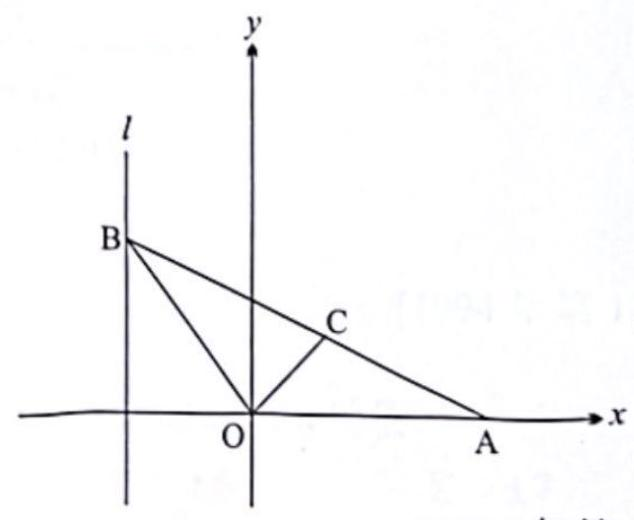
\includegraphics[max width=\textwidth]{2024_06_05_971e6815482d5ecd2718g-26}
    \end{center}
  \begin{enumerate}
    \item 试求 $C$ 点的轨迹方程式, 并指出其 $x$ 与 $y$的限制范围。
    \item 试讨论(a)中所求得的方程式所表示的曲线类型与 $a$ 值的关系。
  \end{enumerate}
\end{enumerate}

\section*{[5.2] 抛物线}
\section*{(选择题)}
\begin{enumerate}
  \item 抛物线 $y^{2}-4 y=4 x$ 的焦点其座标是 
  \item 试求一抛物线之方程式, 其焦点为 $(2,2)$, 准线为 $x+y=0$ 。
  \item 下列哪一曲线与直线 $x+y=0$ 恰有两个交点?
  \item 求抛物线 $y=2 x^{2}-4 x+3$ 的焦点之坐标。
  \item 倾斜角为 $\dfrac{\pi}{3}$ 的直线通过抛物线 $y^{2}=6 x$ 的焦点 $F$, 并交抛物线於 $A$ 及 $B$ 两点。求 $|AB|$ 。
  \item $(y-1)(y-3)=x-2$ 是一条抛物线。问它的顶点的坐标是多少?
  \item 求抛物线 $y^{2}-4 x-2 y-7=0$ 的焦点。
\end{enumerate}

\section*{(作答题)}
\begin{enumerate}
  \item \begin{enumerate}
    \item 试求抛物线 $y=x^{2}+4 x$ 的焦点及准线。
    \item 试绘此抛物线之图像。
  \end{enumerate}
  \item 已知抛物线 $y^{2}=4 x$ 上两点 $A$ 及 $B$, 如果 $OAB$ 是一个等边三角形, 其中 $O$ 是原点,求 $\triangle OAB$ 的面积。
  \item 一抛物线的对称轴垂直于 $y$ 轴。若该抛物线通过三个点 $(7,2),(1,0)$ 及 $(7,-6)$, 求抛物线的方程式及其焦点的坐标。
\end{enumerate}

\section*{[5.3] 椭圆}
\section*{(选择题)}
\begin{enumerate}
  \item 求椭圆 $5 x^{2}+9 y^{2}-20 x-54 y+56=0$ 之中心。
  \item 若椭圆之方程式为 $\dfrac{x^{2}}{16}+\dfrac{y^{2}}{9}=1$, 则其离心率 $e=$ ?
  \item 一椭圆之两焦点为 $(2,1)$ 及 $(6,1)$ 。若其离心率为 $\dfrac{2}{3}$, 试求此椭圆之方程式。
  \item 求以 $(2,-1)$ 为焦点, $x-y+1=0$ 为准线及离心率为 $\dfrac{1}{2} \sqrt{2}$ 的椭圆方程式。
  \item 椭圆 $\dfrac{(x+1)^{2}}{4}+y^{2}=1$ 与拖物线 $y=1-(x+1)^{2}$ 的交点的个数是 $\qquad$
  \item $ABCD$ 是椭圆 $x^{2}+2 y^{2}-4 x+4 y-6=0$ 的内接长方形。已知 $A(4,-3)$, 求 $C$ 的坐标。
  \item 直线 $y=x+k$ 经过椭圆 $x^{2}+9 y^{2}-4 x+18 y+4=0$ 的中心。 $k$ 的值是 $\qquad$ .
  \item 求棈圆 $\dfrac{(x+2)^{2}}{25}+\dfrac{(y-3)^{2}}{16}=1$ 的两个焦点的距离。
  \item 在平面上, 方程式 $\left|\begin{array}{ccc}5 x & x & -5 y \\ 0 & 1 & 6 \\ y & 0 & x\end{array}\right|=8$ 的图象是什么?
  \item 若 $F_{1}$ 及 $F_{2}$ 是椭圆 $\dfrac{x^{2}}{4}+\dfrac{y^{2}}{3}=1$ 的两焦点, 求 $F_{1} ~F_{2}$ 的长。
  \item 若椭圆 $4 x^{2}+y^{2}=k$ 两点间的最长距离是 8 , 求 $k$ 的值。
  \item 若 $F$ 与 $F^{\prime}$ 是㮋圆 $\dfrac{x^{2}}{a^{2}}+\dfrac{y^{2}}{b^{2}}=1(a>b)$ 的焦点。 $P$ 是椭圆上的任意一个点, 则 $PF+PF^{\prime}=$ ?
  \item 如果椭圆的一个焦点将其长轴分成 $5: 3$, 求此椭圆的离心率。
  \item 右图所示, $F$ 及 $F^{\prime}$ 为椭圆 $9 x^{2}+25 y^{2}=225$ 的两个焦点, $B$ 及 $B^{\prime}$ 为椭圆在短轴上的端点。求阴影部分的面积。

\begin{center}
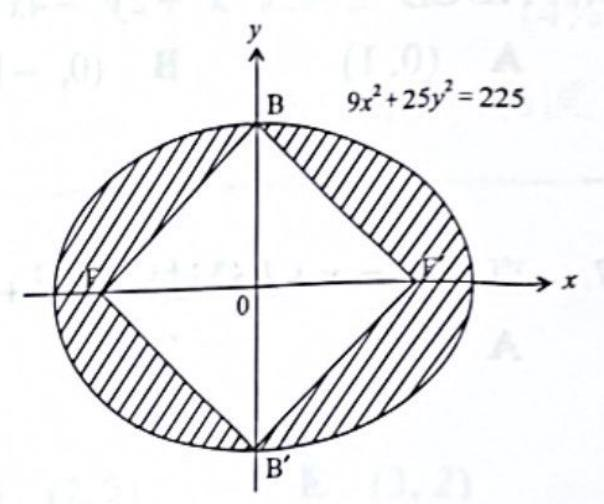
\includegraphics[max width=\textwidth]{2024_06_05_971e6815482d5ecd2718g-30}
\end{center}
\end{enumerate}

\section*{(作答题)}
\begin{enumerate}
  \item $P$ 是焦点为 $S$ 及 $S^{\prime}$ 的椭圆 $\dfrac{x^{2}}{a^{2}}+\dfrac{y^{2}}{b^{2}}=1$ 上的一点。试证 $SP+SP=2 a$ 。
  \item 过椭圆 $x^{2}+2 y^{2}=2$ 的焦点引一条斜率为 1 的直线与椭圆交于 $A$ 及 $B$ 两点。 $O$ 是椭圆的中心, 求 $\triangle OAB$ 的面积。
  \item $P$ 为椭圆上任意一点, $F_{1}$ 与 $F_{2}$ 为其焦点, 试证 $PF_{1}$ 与 $PF_{2}$ 的和等于长轴的长。

  \item \begin{enumerate}
    \item 假设一颗行星绕太阳运行的轨迹是一个半长轴为 $a$ 、离心率为 $e$ 的椭圆。验证

    \begin{enumerate}
      \item 行星离太阳最近的距离是 $r=a(1-e)$;
      \item 行星离太阳最远的距离是 $r=a(1+e)$ 。
    \end{enumerate}
    
    \item 已知哈雷彗星的轨迹为一椭圆, 它的长轴的长为 $36.18 Au$, 短轴的长为 $9.12 Au$ 。求
    
    \begin{enumerate}
      \item 哈雷彗星的离心率;
      \item 哈雷彗星离太阳最近的距离;
      \item 哈雷彗星离太阳最远的距离。
    \end{enumerate}
  \end{enumerate}
  \item 以原点为中心的一椭圆, 其离心率为 $\dfrac{\sqrt{3}}{2}$, 且长轴附在 $x$ 轴上。倘若 $P\left(0, \dfrac{3}{2}\right)$ 为一外点,而 $Q$ 为椭圆上的一点, 使得 $PQ$ 最长的距离为 $\sqrt{7}$, 求
  \begin{enumerate}
    \item 此椭圆的方程;
    \item $Q$ 的坐标。
  \end{enumerate}
  \item 已知椭圆对称于 $x$ 及 $y$ 二轴, 且通过点 $(2,4)$ 。如果椭圆的长轴是短轴的 3 倍, 其中长轴平行于 $x$ 轴, 求这个椭圆的方程式。

  \item 设 $A(-\alpha, 0)$ 及 $B(\alpha, 0)$ 为 $x$ 轴上的两点。一以 $A$ 为中心, $r_{A}$ 为半径的定圆完全在一以 $B$ 为中心, $r_{B}$ 为半径的定圆内。若一动圆同时与此二定圆相切,

  \begin{enumerate}
    \item 求此动圆的圆心的轨迹方程式;
    \item 试证此动圆圆心的轨迹是一以 A、B 为焦点的椭圆。
  \end{enumerate}


  \item 如右图所示, $P(a \cos \theta, b \sin \theta)$ 是椭圆 $\dfrac{x^{2}}{a^{2}}+\dfrac{y^{2}}{b^{2}}=1$ 上的一点。 $Q$ 是椭圆上的另一点使得 $P Q$ 垂直于椭圆的长轴。椭圆在 $P$ 点的法线 $L$ 与直线 $O Q$ 相交于 $R$ 点, $M$ 为 $P R$ 的中点。
  \begin{center}
    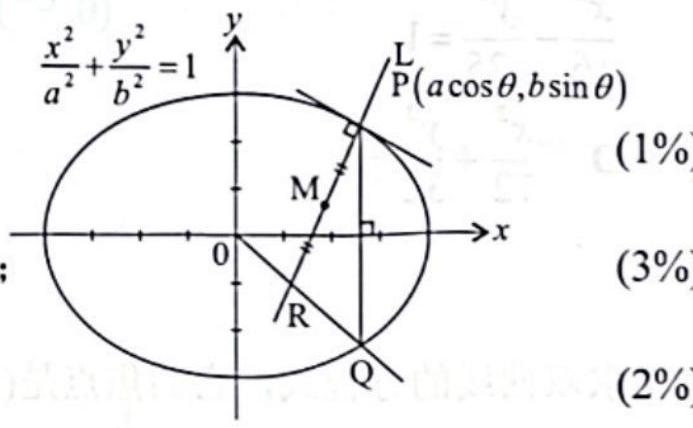
\includegraphics[max width=\textwidth]{2024_06_05_971e6815482d5ecd2718g-31}
    \end{center}

\begin{enumerate}
  \item 求 $OQ$ 的方程式;
  \item 证明 $L$ 的方程式为 $y=\dfrac{a \sin \theta}{b \cos \theta} x+\dfrac{b^{2}-a^{2}}{b} \sin \theta$;
  \item 求 $R$ 点的坐标;
  \item 证明 $M$ 的轨迹方程式为 $\dfrac{x^{2}}{a^{6}}+\dfrac{y^{2}}{b^{6}}=\dfrac{1}{\left(a^{2}+b^{2}\right)^{2}}$ 。
\end{enumerate}

\end{enumerate}

\section*{[5.4] 双曲线}
(选择题)

\begin{enumerate}
  \item 求焦点为 $(-1,1)$, 准线为 $x-y+1=0$, 离心率为 2 之双曲线的方程式。
  \item 双曲线 $x^{2}-y^{2}=4$ 的渐近线其方程式是 $\qquad$ .
  \item 中心为 $(1,0)$ 的一个等轴双曲线通过点 $P(4,0)$ 。它的其中一条渐近线是 $x-y-1=0$ 。试求这个等轴双曲线的方程式。
  \item 一双曲线通过点 $M(-9,2)$, 且它的两条浙近线是 $y= \pm \dfrac{2}{3} x$ 。求此双曲线的方程式。
  \item 求双曲线的方程式, 它的焦点是 $(1,2)$, 准线是 $3 x-4 y+1=0$ 及离心率是 $\dfrac{5}{2}$ 。
  \item 若一双曲线的顶点为 $(2,0)$ 及 $(-2,0)$, 焦点为 $(5,0)$ 及 $(-5,0)$, 求其渐近线的方程式。
  \item 已知一椭圆的顶点和焦点分别是双曲线 $\dfrac{x^{2}}{16}-\dfrac{y^{2}}{9}=1$ 的焦点和顶点, 求此椭圆的方程式。
  \item 已知 $\dfrac{x^{2}}{a^{2}-3}+\dfrac{y^{2}}{2 a}=1$ 为一直角双曲线且其准线平行于 $x$ 轴, 求 $a$ 的值。
  \item 已知一双曲线的两条渐近线为 $4 x+3 y=0$ 及 $4 x-3 y=0$ 。若 $y=\dfrac{32}{5}$ 是其中一条准线, 求此双曲线的顶点坐标。
  \item 求双曲线 $-\dfrac{x^{2}}{5}+\dfrac{(y+2)^{2}}{4}=1$ 的准线方程式。
  \item 求两条曲线 $\dfrac{x^{2}}{9}+\dfrac{y^{2}}{4}=1$ 与 $\dfrac{(x+1)^{2}}{16}-\dfrac{y^{2}}{9}=1$ 的交点个数。
\end{enumerate}

(作答题)

\begin{enumerate}
  \item 试证双曲线 $\dfrac{x^{2}}{a^{2}}-\dfrac{y^{2}}{b^{2}}=1$ 上任一点至二渐近线距离之积为一定值。
  \item 一直线的参数方程式为 $\left\{\begin{array}{l}x=2+t \\ y=\sqrt{3} t\end{array}\right.$, 式中 $t$ 为参数。求此直线在双曲线 $x^{2}-y^{2}=1$ 上截得的弦长。
  \item 已知以原点为中心的双曲线的一个焦点是 $(\sqrt{2}, 0)$, 它的相应的准线是 $x=\dfrac{1}{\sqrt{2}}$, 求此双曲线的标准方程式。
  \item 已知 $A(27,1)$ 及 $B(9,3)$ 是直角双曲线 $x y=27$ 上的两点, 延长弦 $AB$ 分别交 $x$ 及 $y$ 二轴于 $P$ 及 $Q$ 两点。证明
  \begin{enumerate}
    \item $PQ$ 的长度是 $AB$ 的长度的两倍;
    \item 直线 $AB$ 与另一个直角双曲线 $x y=36$ 相切; 并求其切点。
  \end{enumerate}
  \item 如右图所示, A、B 是双曲线 $\dfrac{x^{2}}{a^{2}}-\dfrac{y^{2}}{b^{2}}=1$ 上任意两点, $M(p, q)$ 是 $AB$ 的中点。试证直线 $AB$ 的方 程 式为 $y-q=\dfrac{b^{2} p}{a^{2} q}(x-p)$ 。

\begin{center}
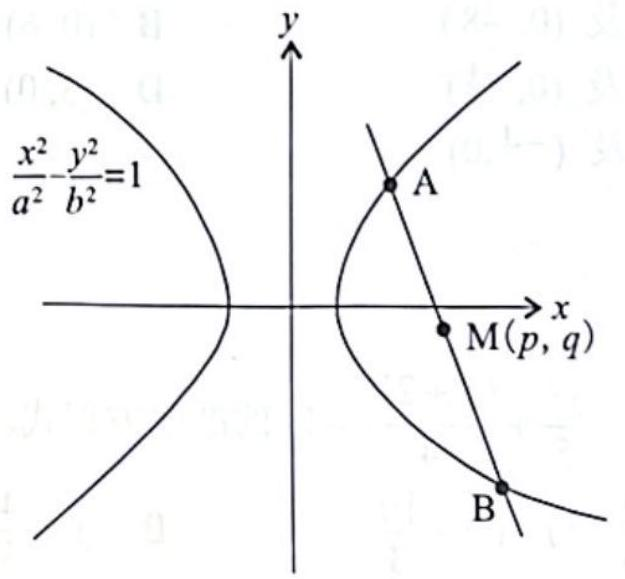
\includegraphics[max width=\textwidth]{2024_06_05_971e6815482d5ecd2718g-34}
\end{center}

  \item 一平行于 $x$ 轴的直线通过双曲线 $\dfrac{y^{2}}{a^{2}}-\dfrac{x^{2}}{b^{2}}=1$ 的一个焦点并交该双曲线于 $A$ 及 $B$ 两点。求 $AB$ 的长。

  \item 已知一双曲线的浙近线方程式是 $x+2 y-1=0$ 及 $x-2 y-1=0$ 。若双曲线的虚轴长为 2 单位且与 $y$ 轴平行, 求此双曲线的方程式。

  \item 右图所示的曲线为双曲线 $\dfrac{y^{2}}{9}-\dfrac{x^{2}}{16}=1$在 $y>0$ 的部份。 $F$ 是焦点, $L$ 是准线。 $A\left(x_{a}, y_{a}\right), B\left(\dfrac{15}{2}, \dfrac{51}{8}\right), C\left(x_{c}, y_{c}\right)$ 是曲线上的三点。

  \begin{enumerate}
    \item 求 $F$ 的坐标和 $L$ 的方程式;

    \item 若线段 $AF, BF, CF$ 的长成等差数列, 证明 $y_{a}+y_{c}=\dfrac{51}{4}$ 。
  \end{enumerate}

\begin{center}
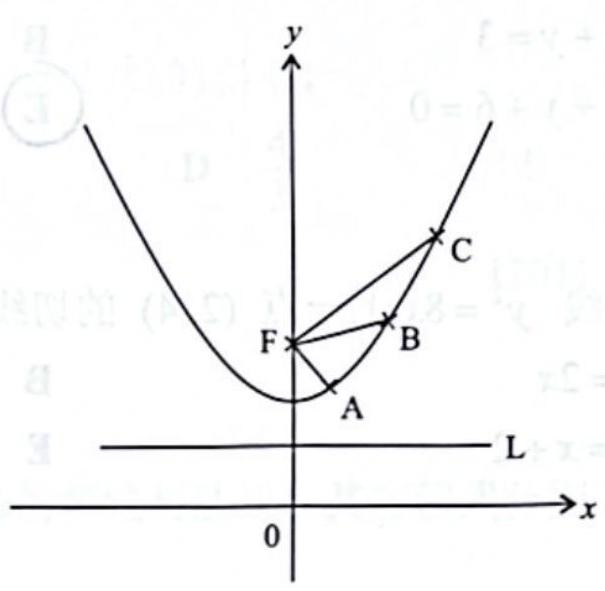
\includegraphics[max width=\textwidth]{2024_06_05_971e6815482d5ecd2718g-35}
\end{center}
\end{enumerate}


\end{document}